\chapter{Esperimenti}

Per il perseguimento dello scopo di questa tesi si è deciso  di utilizzare un approccio con reti neurali convoluzionali basato sull'architettura delle Fully Convolutional Networks esposte nel capitolo precedente. Verranno dunque qui mostrate le motivazioni di questa scelta, l'evoluzione del metodo sviluppato e varie considerazioni sui risultati ottenuti.

\section{Descrizione del metodo}
Recentemente, come già accennato, l'architettura delle FCN si è dimostrata un mezzo potente per il rilevamento di oggetti nelle immagini, rendendo superflua la fase di \textit{region proposal} e ponendo in ombra metodi per la localizzazione multipla basati su RRCN.\par
È naturale quindi porsi la domanda di dove può arrivare la potenza di queste reti per task diversi da quelli per cui sono state concepite, ricordando che alla base vi è un generico classificatore.\par
Il nostro obiettivo è quello di trovare aree di testo in immagini digitali, quindi qualcosa che va al di là della semplice concezione di \textit{oggetto}. Un testo può infatti essere presente su una varietà immensa di oggetti eterogenei, basti pensare ai cartelli stradali, ai giornali, alle magliette oppure agli schermi di televisori e smartphone.\par
Pare dunque impossile definire un oggetto singolo classificabile come testo, se non pensando di isolare singolo carattare, obiettivo che ci viene reso impossibile dall'indisponibilità di un dataset adeguato.\par
Nonostante tutto, invece questa concezione astratta può venire superata dalle reti neurali attraverso un corretto addestramento date le giuste informazioni. A prova di ciò possiamo citare~\cite{pixellevel}, dove per localizzare le singole istanze di vari oggetti vengono utilizzate due FCN aggiuntive, una per la predizione della profondità e l'altra per la direzione dal centroide di ogni istanza. Si veda l'immagine~\ref{fig:pixellevel} per un'esempio della groundtruth.

\begin{figure}[H]
	\centering
	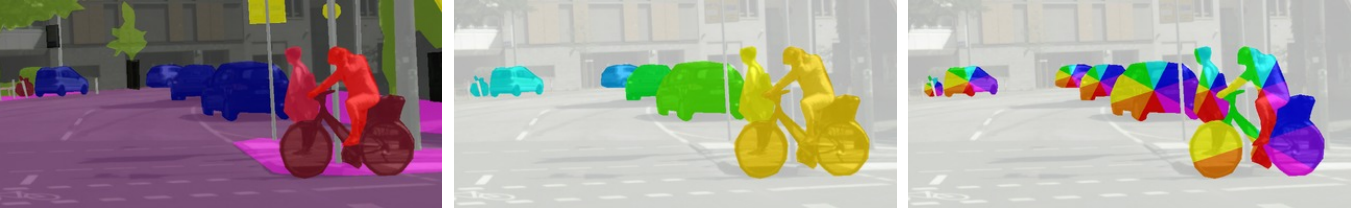
\includegraphics[width=\textwidth]{pixellevel.png}
	\caption{Esempi delle groundtruth.}
\label{fig:pixellevel}
\end{figure}

I più che discreti risultati di questo lavoro ci dimostrano dunque la grande versatilità di una FCN per un grade campo di mansioni che esulano da quello della loro concezione originale.

Assodato il fatto che verrà utilizzata una FCN per la segmentazione di un'immagine in area di testo e non, di seguito verrà descritto il processo di sviluppo della nostra pipeline per la localizzazione per poi confrontarci con metodi concorrenti.


\subsection{Strumenti}
Python\cite{python} si è imposto negli anni come linguaggio molto semplice da usare per la prototipizzazione di algoritmi nonostante la sua lentezza dovuta alla sua natura di linguaggio interpretato. Questa sua debolezza è però stata in parte superata grazie a moduli sviluppati come \textit{wrapper} intorno a librerie scritte in linguaggi compilati come C/C++, rendendo dunque più accessibile e semplificato l'utilizzo di routine altamente efficenti.\par
Tra le più famose, ed utilizzate in questa tesi, citiamo \textbf{NumPy}\cite{numpy} per la manipolazione di array multidimensionali, \textbf{SciPy}\cite{scipy} per gli algoritmi matematici più vari, \textbf{OpenCV}\cite{opencv} per l'elaborazione di immagini ed infine \textbf{Shapely}\cite{shapely} per la manipolazione di oggetti geometrici.\par
Per l'implementazione della \textit{Fully Convolutional Network} però ci si è affidati a \textbf{TensorFlow}\cite{tensorflow}, una libreria per l'implementazione, visualizzazione e profilazione di reti neurali sviluppata da Google dal 2015.


\subsection{Groundtruth}
%La definizione di una groundtruth è una fase estremamente importante in quanto da questa dipende tutto il processo di addestramento del nostro modello e l'estrapolazione finale dei dati a noi rilevanti.\par
L'output desiderato della nostra rete consiste in un'immagine delle stesse dimensioni di quella di input segmentata in due classi: testo e ``non testo'', quindi come prima idea potrebbe sovvenire quella di specificare, lettera per lettera, le aree di testo rispetto al background. Ciò potrebbe sembrare l'approccio migliore atto a generare risultati accuratissimi non solo per la localizzazione, ma anche per la segmentazione delle singole lettere per il successivo task di riconoscimento del testo, ma ad oggi non esistono dataset simili a nostra disposizione.\par
Il passo successivo è quindi quello di generalizzare l'idea precedente portando l'area di interesse non quindi alla forma della singola lettera, ma la sua posizione. Il dataset SynthText introdotto nella sezione~\ref{subsec:synth} viene in nostro soccorso, essendo infatti un dataset sintetico ci mette a disposizione questi dati specifici fornendo le bounding box per ogni carattere.\par
Per quanto riguarda gli altri dataset introdotti in precedenza, le loro annotazioni ci forniscono solo i dati approssimativi di una bounding box per parola, quindi possiamo ancora astrarre e considerare quelle zone come area di interesse, seppur aggiungendo teoricamente molto più rumore.\par


\subsection{Iperparametri}
La scelta di iperparametri per l'ottimizzazione di una rete neurale è una delle sfide maggiori che si affrontano durante la fase di addestramento di un modello. Di seguito sono elencati quelli principali individuati durante le fasi preliminari di preparazione della rete:
\begin{description}
	\item[Batch size:]
		Un numero maggiore velocizza l'apprendimento. $16$ è il massimo che si è potuto raggiungere rimanendo nei limiti di memoria a disposizione.
	\item[Learning rate:]
		Influenzato dal batch size, nonostante l'utilizzo di algoritmi sofisticati per la discesa del gradiente, valori troppo grandi ($10^{-4}$) non portano a nessuna predizione, mentre valori troppo piccoli ($10^{-6}$) rallentano l'apprendimento. $10^{-5}$ è il valore utilizzato per tutti gli esperimenti a seguire con Adam.
	\item[Loss function:]
		Pixelwise Softmax Cross-Entropy con azzeramento del valore di loss su zone con testo contrassegnato come illeggibile dai dataset in uso.
\end{description}


\subsection{Dettagli preliminari}

Prima di procedere con l'analisi dei vari esperimenti svolti è necessario chiarire alcuni punti riguardanti implementazione della rete, gestione dell'apprendimento, estrazione delle predizioni finali e utilizzo dei vari dataset.\par

\subsubsection{FCN}
\label{subsec:impl}
Qui elencate le caratteristiche principali dell'architettura: 
\begin{itemize}
	\item \textit{FCN-8} (3 deconvoluzioni con addizione di due layer di pooling come illustrato in figura~\ref{fig:fcn})
	\item \textit{VGG19} come classificatore con pesi già addestrati per ImageNet~\cite{pretrained}
	\item \textit{ReLU} standard
	\item \textit{Max Pooling}
	\item \textit{Padding} nell'ultima convoluzione della VGG per facilitare l'utilizzo della rete neurale su immagini di dimensione variabile
\end{itemize}


\subsubsection{Generazione dati di training}
\label{subsubsec:gendata}
Poiché le immagini dei vari dataset presentano risoluzioni pressoché sempre differenti, è necessario definire un metodo per ottenere zone di grandezza fissa da ciascuna di esse in modo da adoperare un batch size maggiore di 1.\par
L'idea di estrarre una zona randomica, seppur molto semplice, potrebbe rallentare l'addestramento in quanto, come già analizzato in figura~\ref{fig:annratio}, le zone di testo occupano un'area decisamente esigua rispetto all'immagine in cui compaiono, abbassando dunque le probabilità che possano essere incluse nel nostro ``ritaglio'' randomico.\par
La soluzione adottata consiste dunque nel partire da un'annotazione contrassegnata come leggibile e da lì espandere randomica la selezione verso i bordi dell'immagine, squadrarla (anche uscendo dai limiti) ed infine ridimensionare l'area selezionata alla risoluzione prefissata.\par
Questo approccio ha un grande pregio, infatti per ogni immagine di partenza potrebbero essere create decine di esempi differenti, estendendo di conseguenza il dataset di base.\par
L'algoritmo sviluppato è presentato nello pseudocodice~\ref{alg:gendata}.


\begin{algorithm}
\begin{algorithmic}
	\Function{GetImage}{$\textit{img, annGt, weightGt, id, cropSize}$}
		\State{$\textit{annotation} \gets \Call{Random}{\Call{Annotations}{\textit{id}}}$}
		\LineComment{Espandi la bounding box verso i bordi.}
		\State{$x_1, x_2, y_1, y_2 \gets \textit{annotation.bbox}$}
		\State{$x_1 \gets x_1 - \Call{Random}{0 \ldots x_1}$}
		\State{$y_1 \gets y_1 - \Call{Random}{0 \ldots y_1}$}
		\State{$x_2 \gets x_2 + \Call{Random}{0 \ldots \textit{img.width}  - x_2}$}
		\State{$y_2 \gets y_2 + \Call{Random}{0 \ldots \textit{img.height} - y_2}$}
		\State{$\textit{ratio} \gets (x_2 - x_1) / (y_2 - y_1)$}
		\LineComment{Modifica le coordinate in modo da ottenere un quadrato.}
		\If{$\textit{ratio} > 1$}
			\State{$\textit{diff} \gets (x_2 - x_1) - (y_2 - y_1)$}
			\State{$\textit{split} \gets \Call{Random}{0 \ldots \textit{diff}}$}
			\State{$y_1 \gets y_1 - \textit{split}$}
			\State{$y_2 \gets y_2 + (\textit{diff} - \textit{split})$}
		\ElsIf{$\textit{ratio} < 1$}
			\State{$\textit{diff} \gets (y_2 - y_1) - (x_2 - x_1)$}
			\State{$\textit{split} \gets \Call{Random}{0 \ldots \textit{diff}}$}
			\State{$x_1 \gets x_1 - \textit{split}$}
			\State{$x_2 \gets x_1 + (\textit{diff} - \textit{split})$}
		\EndIf{}
		\LineComment{Ottieni i valori di padding nel caso si esca dai limiti.}
		\State{$\textit{pad}_y \gets ( \max(0, -y_1),\; \max(0, y_2 - \textit{img.height}) )$}
		\State{$\textit{pad}_x \gets ( \max(0, -x_1),\; \max(0, x_2 - \textit{img.width}) )$}
		\State{$x_1 \gets \max(0, x_1)$} 
		\State{$y_1 \gets \max(0, y_1)$}
		\LineComment{Per ogni immagine (originale, groundtruth e pesi)}
		\LineComment{ritaglia, aggiungi padding e applica resize.}
		\ForAll{$\textit{element} \in [img, annGt, weightGt]$}
			\State{$\textit{element} \gets \textit{element}[y_1 \ldots y_2][x_1 \ldots x_2]$}
			\State{$\textit{element} \gets \Call{Pad}{\textit{element, pad}_x \textit{, pad}_y}$}
			\State{$\textit{element} \gets \Call{Resize}{\textit{element, cropSize}}$}
		\EndFor{}
		\Return{$img, annGt, weightGt$}
	\EndFunction{}
\end{algorithmic}
\caption{Generazione dati di training}
\label{alg:gendata}
\end{algorithm}


\subsubsection{Predizioni}
Partendo dal presupposto che il risultato finale su cui operare sia un'immagine binaria in cui le zone ``attive'' rappresentano una predizione di un'area di testo, ciò che si andrà a fare per estrarre le bounding box in breve è quanto segue:
\begin{itemize}
	\item operazione morfologica di closing con una maschera $3\times3$ 
	\item labeling delle componenti connesse con maschera $3\times3$ completa 
	\item eliminazione delle c.c.\ con un'area minore di una certa soglia 
	\item estrazione della bounding box (ruotata o meno in base al test set) da ciascuna componente connessa
\end{itemize}

Lo pseudocodice~\ref{alg:bbox} illustra l'algoritmo.

\begin{algorithm}
\caption{Estrazione delle bounding box da immagine binaria}
\label{alg:bbox}
\begin{algorithmic}
	\Function{GetPredictions}{$\textit{img, threshold}$}
		\State{$\textit{img} \gets \Call{closing}{\textit{img}}$}
		\LineComment{Trova le componenti connesse}
		\State{$\textit{labeled, nlabels} \gets \Call{label}{\textit{img}}$}
		\State{$\textit{bboxes} \gets \emptyset$}
		\If{$\textit{nlabels} > 0$}
			\LineComment{Date le componenti connesse, ottieni le loro aree}
			\State{$\textit{areas} \gets \{ \Vert \textit{labeled}[\textit{labeled} = i] \Vert \mid i \textbf{ from } 1 \textbf{ to } \textit{nlabels} \} $}
			\For{$i \textbf{ from } 1 \textbf{ to } \textit{nlabels}$}
				\If{$\textit{areas}[i] \geq \textit{threshold}$}
					\State{$\textit{lone} \gets \textbf{copy } \textit{labeled}$}
					\LineComment{Isola una componente connessa}
					\State{$\textit{lone}[\textit{lone} \neq i] \gets 0$}
					\State{$\textit{cnt} \gets \Call{FindContour}{\textit{lone}}$}
					\LineComment{per estrarne la bounding box}
					\State{$\textit{bboxes} \gets \textit{bboxes} \cup \{\Call{BoundingBox}{\textit{cnt}}\} $}
				\EndIf{}
			\EndFor{}
		\EndIf{}
		\Return{$\textit{bboxes}$}
	\EndFunction{}
\end{algorithmic}
\end{algorithm}


\subsubsection{Dataset}
Non è stato possibile utilizzare COCO-Text in fase di testing in quanto i risultati pubblici non sono ancora disponibili in data di stesura di questa tesi, mentre SynthText non dispone di sottoinsieme di testing prefissato.\par
Focused Scene Text è stato ignorato per la fase di training poiché presenta pochi dati che si possono facilmente ritrovare in Incidental Scene Text.\par

\begin{table}[H]
\centering
\begin{threeparttable}
	\begin{tabular}{l*{3}{c}}
		\toprule
		& Training	& Validation\footnotemark[1] & Testing\footnotemark[2] \\
		\midrule
		COCO-Text				& $\bullet$	& $\bullet$	&           \\
		SynthText				& $\bullet$	&			&           \\
		Incidental Scene Text	& $\bullet$	&			& $\bullet$	\\
		Focused Scene Text		&          	&			& $\bullet$ \\
		\bottomrule
	\end{tabular}
	\begin{tablenotes}
		\small
		\item
			$^{1}$ Comparazione fra modelli addestrati diversamente
		\item
			$^{2}$ Confronto finale con metodi di terzi
	\end{tablenotes}
\end{threeparttable}
\end{table}



\section{Addestramento sui dataset}


\subsection{COCO-Text}
\label{subsec:train_coco}
Questo dataset, nonostante le sue imprecisioni, comincia subito a produrre risultati visivamente coerenti e significativi, come mostrato nella seguente immagine~\ref{fig:coco_example}.\par

\begin{figure}[H]
	\centering
	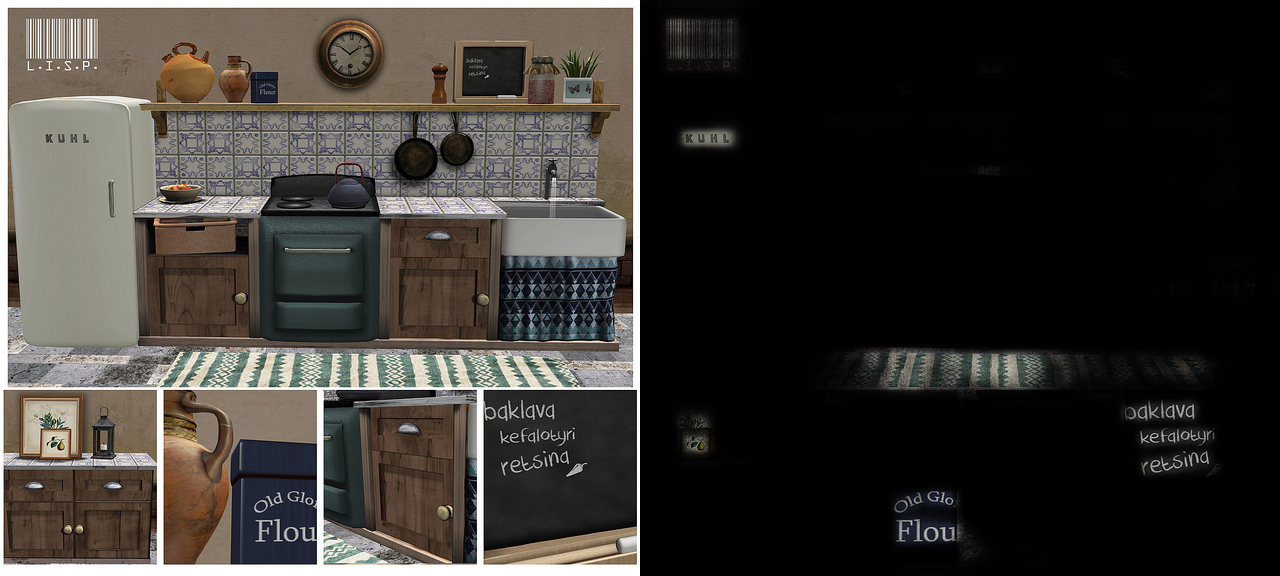
\includegraphics[width=\textwidth]{coco60kpred.png}
	\caption{Immagine originale e immagine combinata con mappa delle probabilità.}
\label{fig:coco_example}
\end{figure}

Osservando l'andamento della loss per tutte e le iterazioni si può notare un trend che farebbe pensare ad un overfitting sui dati, infatti da 60mila iterazioni in poi (circa 64 epoche\footnote{nonostante parlare di epoche abbia poco senso in quanto, come già spiegato nella sezione~\ref{subsubsec:gendata}, il training set è mutevole}) la loss su un sottoinsieme fisso del validation set rimane pressoché invariata mentre quella del training è in lenta discesa.

\begin{figure}[H]
	\centering
	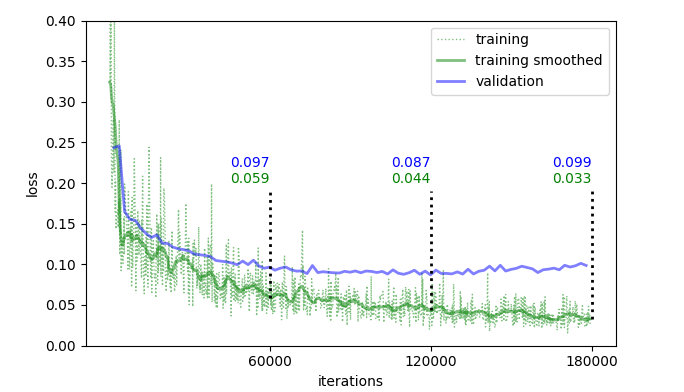
\includegraphics[width=\textwidth]{coco_loss.png}
	\caption{Curve di loss su training a validation set.}
\label{fig:coco_loss}
\end{figure}

Applicando invece l'algoritmo di estrazione delle bounding box con soglia 32 pixel ed infine valutando con \textit{Intersection over Union} a $0.5$, i miglioramenti vi sono, come si può notare dai risultati riportati nella tabella~\ref{tab:coco}.

\begin{table}[H]
\centering
\begin{threeparttable}
	\begin{tabular}{l*{5}c}
		\toprule
		\multirow{2}{*}{\textbf{Iterazioni}} & \multicolumn{3}{c}{\textbf{Recall}} & \multirow{2}{*}{\textbf{Precision}} & \multirow{2}{*}{\textbf{F1-score}} \\
		\cmidrule(lr){2-4}
		& Leggibili & Illegibili & Totale &  &  \\
		\midrule
		\multicolumn{6}{l}{Intero validation set} \\
		60k		& $16.21$ & $4.14$ & $12.28$ & $13.85$ & $13.01$ \\
		180k	& $20.87$ & $9.59$ & $17.29$ & $17.72$ & $17.50$ \\
		\midrule
		\multicolumn{6}{l}{Almeno un leggibile per immagine} \\
		60k		&   ---   & $3.41$ & $12.79$ & $24.11$ & $16.71$ \\
		180k	&   ---   & $9.00$ & $17.78$ & $28.15$ & $21.79$ \\
		\bottomrule
	\end{tabular}
	\begin{tablenotes}
		\item \footnotesize{Valori espressi in percentuale.}
	\end{tablenotes}
\end{threeparttable}
\caption{}\label{tab:coco}
\end{table}

%Non è ben chiaro dunque l'appiattimento della curva di loss su un sottoinsieme del validation set.


\subsection{Incidental Scene Text}
\label{subsec:train_inc}
I risultati già dopo le prime 60mila iterazioni (960 epoche) non sono promettenti, infatti si presentata un calo drastico nella precision rispetto a COCO-Text. Si confrontino i risultati riportati nella tabella~\ref{tab:incidental} con quelli della precedente tabella~\ref{tab:coco}.

\begin{table}[H]
\centering
\begin{threeparttable}
	\begin{tabular}{l*{5}c}
		\toprule
		\multirow{2}{*}{\textbf{Iterazioni}} & \multicolumn{3}{c}{\textbf{Recall}} & \multirow{2}{*}{\textbf{Precision}} & \multirow{2}{*}{\textbf{F1-score}} \\
		\cmidrule(lr){2-4}
		& Leggibili & Illegibili & Totale &  &  \\
		\midrule
		\multicolumn{6}{l}{Intero validation set} \\
		60k		& $19.07$ & $5.78$ & $14.54$ & $7.87$ & $10.21$ \\
		\midrule
		\multicolumn{6}{l}{Almeno un leggibile per immagine} \\
		60k		&   ---   & $5.69$ & $15.48$ & $13.95$ & $14.67$ \\
		\bottomrule
	\end{tabular}
	\begin{tablenotes}
		\item \footnotesize{Valori espressi in percentuale.}
	\end{tablenotes}
\end{threeparttable}
\caption{}\label{tab:incidental}
\end{table}


Il problema potrebbe essere imputabile alla groundtruth lievemente differente rispetto a quella di COCO-Text la quale presenta poche bounding box ruotate. Più avanti ritorneremo ad analizzare questo fenomeno.


\subsection{SynthText}
L'addestramento su questo dataset viene presto abbandonato ancora in fase sperimentale in quanto i risultati visivi (si veda la figura~\ref{fig:synth_example}) mostrano chiaramente un apprendimento poco significativo.\par

\begin{figure}[H]
	\centering
	\begin{subfigure}[b]{0.49\textwidth}
		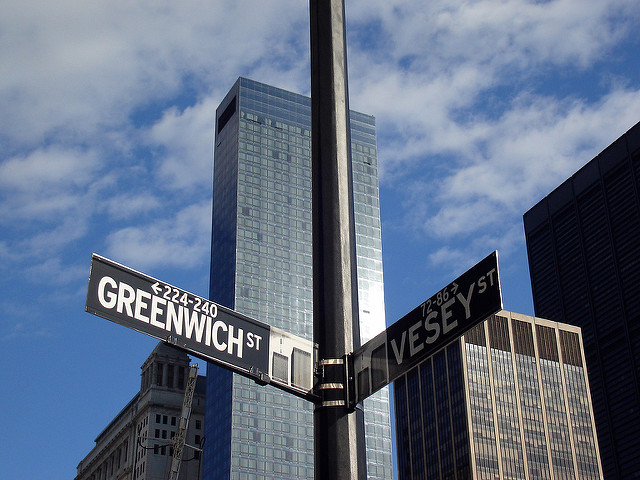
\includegraphics[width=\textwidth]{synth_original.png}
	\end{subfigure}
	\hfill
	\begin{subfigure}[b]{0.49\textwidth}
		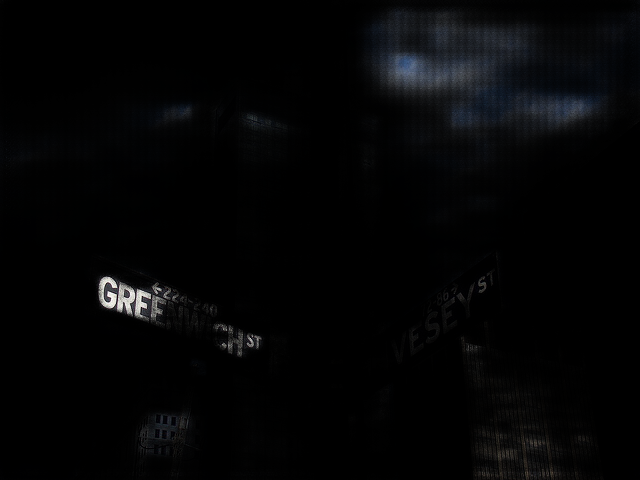
\includegraphics[width=\textwidth]{synth_mask.png}
	\end{subfigure}
\caption{}
\label{fig:synth_example}
\end{figure}

Il problema è molto probabilmente dovuto alla natura sintetica del dataset per cui molti elementi testuali, seppur posizionati tenendo conto della forma e perspettiva, si ritrovano in contesti completamente irreali e risultano dunque fuorvianti ai fini dell'addestramento della rete neurale.



\section{Modifiche strutturali}

I risultati ottenuti, seppur mostrino come questo approccio sia corretto nella forma, non raggiungono numeri soddisfacenti, l'obiettivo è dunque quello di cercare di migliorare senza però complicare il processo di estrazione delle bounding box illustrato nello pseudocodice~\ref{alg:bbox}. Ciò è dato dal fatto che il fine postoci è quello di adoperare principalmente una FCN, senza dunque ricorrere a metodi raffinati da porre in coda alla catena di elaborazione dei dati come effettuato da diversi altri metodi citati in precedenza nella sezione~\ref{sec:sota}.\par
Osservando le predizioni ottenute con l'addestramento su COCO-Text, si può notare come le zone di testo predette non siano molto raffinate e finiscano dunque per raggruppare insieme molte parole vicine fra di loro. Per ovviare a questo problema le soluzioni adottate che andremo a descrivere sono principalmente due:
\begin{itemize}
	\item
		Nuova classe ``bounding box'' che rappresenti il contorno di una parola.
	\item
		Nuova classe ``separazione'' che rappresenti una linea immaginaria che separi due parole vicine fra di loro.
\end{itemize}

In quanto difficilmente una \textit{Fully Convolutional Network} è in grado di generare una segmentazione raffinata in presenza di più classi, soprattutto quando queste sono simili o complementari, la generazione delle predizioni di aree testuali verrà effettuata come descritto nell'algoritmo~\ref{alg:sub_prob}, piuttosto che nel modo tradizionale con il quale si sceglierebbe la classe con score maggiore.

\begin{algorithm}
\caption{}\label{alg:sub_prob}
\begin{algorithmic}
	\State{$\textit{output} \gets \emptyset \in \mathbb{R}^{n \times m}$}
	\Comment{$\textit{probText, probThird} \in \mathbb{R}^{n \times m}$}
	\For{$i \textbf{ from } 1 \textbf{ to } n$}
		\For{$j \textbf{ from } 1 \textbf{ to } m$}
			\State{$\textit{value} \gets \textit{probText}[i][j] - \textit{probThird}[i][j]$}
			\If{$\textit{value} \geq \textit{threshold}$}
				\State{$\textit{output}[i][j] \gets \textit{value}$}
			\EndIf{}
		\EndFor{}
	\EndFor{}
	\Return{$\textit{output}$}
\end{algorithmic}
\end{algorithm}

dove \textit{probText} e \textit{probThird} sono rispettivamente mappe di probabilità di appartenenza alle classi di testo e bounding box / separazione, entrambe generate dopo l'applicazione della funzione di Softmax agli score finali.


\subsection{BranchFCN}
\label{subsec:train_branch}
Questa approccio deve il suo nome alla modifica apportata all'FCN fin'ora usata per contrastare un problema sorto in fase di implementazione. Infatti durante un addestramento preliminare si è notato che con l'introduzione della nuova classe delle bounding box le zone con probabilità di essere testo venivano ristrette producendo come effetto indesiderato l'annichilamento di tali predizioni ove il testo fosse di piccole dimensioni.\par
La soluzione consiste nello sdoppiare la fase di deconvoluzione finale in due rami, uno che generi predizioni per la solo area di testo ed il secondo per le sole bounding box. La scelta di ramificare dopo la fase di classificazione è dettata prettamente dal volere mantenere una certa efficenza, si evita infatti di raddoppiare il numero di pesi totali della rete (presenti perlopiù nella fase finale della VGG) e di addestrare due reti similari separate.\par
In aggiunta a ciò, l'operazione di \texttt{closing} utilizzata nell'algoritmo~\ref{alg:bbox} viene sostituita con un'operazione di \texttt{dilation} al fine di recuperare parte dei contorni persi durante l'applicazione dell'algoritmo~\ref{alg:sub_prob} precedentemente descritto.\par 
Come per il primo training su COCO-Text, anche con questo approccio si è deciso di addestrare la rete per 180mila iterazioni. I risultati visivi sono già da subito promettenti come mostrato nella figura~\ref{fig:branch_visualize}.

\begin{figure}[H]
	\centering
	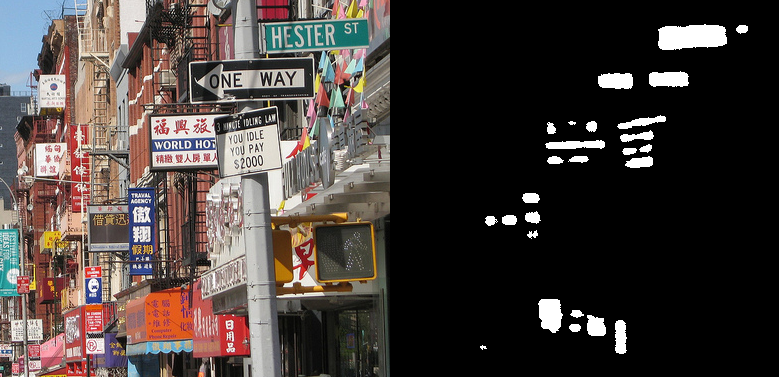
\includegraphics[width=0.9\textwidth]{branch_visualize.png}
	\caption{Immagine con relativa mappa delle probabilità.}
\label{fig:branch_visualize}
\end{figure}

Il grafico della funzione di loss (una media aritmetica fra i due rami dell'architettura) ci mostra come l'apprendimento non venga rallentato dalla presenza di una nuova classe in quanto i valori riflettono quanto già visto con l'addestramento di base su COCO-Text.

\begin{figure}[H]
	\centering
	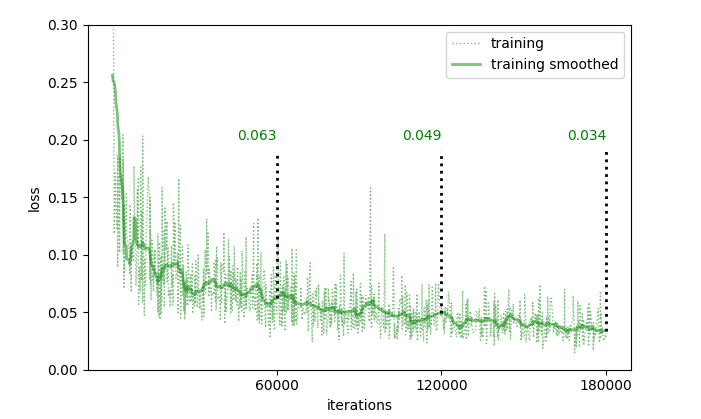
\includegraphics[width=\textwidth]{branch_loss.png}
	\caption{Curva di loss su training set.}
\label{fig:branch_loss}
\end{figure}

Nella tabella seguente~\ref{tab:branch} i risultati sul validation set, nella quale si può notare come i miglioramenti generali rispetto all'addestramento base siano notevoli seppur vi sia un lieve decremento nella recall su zone illeggibili.


\begin{table}[H]
\centering
\begin{threeparttable}
	\begin{tabular}{l*{5}c}
		\toprule
		\multirow{2}{*}{\textbf{Iterazioni}} & \multicolumn{3}{c}{\textbf{Recall}} & \multirow{2}{*}{\textbf{Precision}} & \multirow{2}{*}{\textbf{F1-score}} \\
		\cmidrule(lr){2-4}
		& Leggibili & Illegibili & Totale &  &  \\
		\midrule
		\multicolumn{6}{l}{Intero validation set} \\
		180k		& $35.91$ & $6.98$ & $26.13$ & $21.55$ & $23.62$ \\
		\midrule
		\multicolumn{6}{l}{Almeno un leggibile per immagine} \\
		180k		&   ---   & $6.74$ & $27.99$ & $35.46$ & $31.29$ \\
		\bottomrule
	\end{tabular}
	\begin{tablenotes}
		\item \footnotesize{Valori espressi in percentuale.}
	\end{tablenotes}
\end{threeparttable}
\caption{}\label{tab:branch}
\end{table}


\subsection{Word Division}
\label{subsec:train_wd}
Come approccio alternativo rimane quello di introduzione di una classe che rappresenti una linea immaginaria di separazione fra due parole abbastanza vicine. A differenza di BranchFCN però qui non è necessario modificare la rete neurale poiché, per come definita, la nuova classe non dovrebbe avere effetti collaterali sulle predizioni delle aree di testo.\par
V'è però il problema della definizione di un algoritmo per il posizionamento di questa nuova classe nell'immagine di groundtruth. La seguente figura~\ref{fig:division_proto} dovrebbe chiarire l'idea alla base dello pseudocodice~\ref{alg:drawsep}, il cui scopo è quello di rilevare i punti di intersezione esterni di due bounding box, compiendo delle espansioni qualora non fossero in contatto diretto.

\begin{figure}[H]
	\centering
	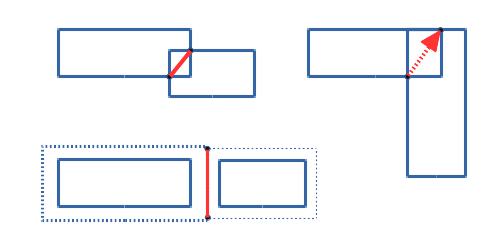
\includegraphics[width=0.8\textwidth]{division_proto.png}
	\caption{I tre esempi principali di estrazione della linea di separazione.}
\label{fig:division_proto}
\end{figure}

Nella seguente tabella~\ref{tab:word} i risultati sul validation set, non dissimili a quelli osservati in precedenza con BranchFCN.\par

\begin{table}[H]
\centering
\begin{threeparttable}
	\begin{tabular}{l*{5}c}
		\toprule
		\multirow{2}{*}{\textbf{Iterazioni}} & \multicolumn{3}{c}{\textbf{Recall}} & \multirow{2}{*}{\textbf{Precision}} & \multirow{2}{*}{\textbf{F1-score}} \\
		\cmidrule(lr){2-4}
		& Leggibili & Illegibili & Totale &  &  \\
		\midrule
		\multicolumn{6}{l}{Intero validation set} \\
		180k		& $38.88$ & $8.37$ & $28.70$ & $23.64$ & $25.94$ \\
		\midrule
		\multicolumn{6}{l}{Almeno un leggibile per immagine} \\
		180k		&   ---   & $7.84$ & $30.60$ & $36.74$ & $33.39$ \\
		\bottomrule
	\end{tabular}
	\begin{tablenotes}
		\item \footnotesize{Valori espressi in percentuale.}
	\end{tablenotes}
\end{threeparttable}
\caption{}\label{tab:word}
\end{table}


\begin{algorithm}[H]
\begin{algorithmic}
\caption{Calcolo e disegno linee di separazione.}\label{alg:drawsep}
\Function{DrawSeparations}{$\textit{gtImage, bboxes, nExpansion, thickness}$}
	\State{$\textit{intersected} \gets \emptyset$}
	\For{$i \textbf{ from } 0 \textbf{ to } \textit{nExpansion}$}
		\For{$b_1 \in \textit{bboxes}$}
			\For{$b_2 \in \textit{bboxes}$}
				\If{$(b_1, b_2) \notin \textit{intersected}$}
					\State{$\textit{line} \gets \Call{GetLine}{b_1 \textit{, } b_2}$}
					\If{$\textit{line} \neq \varnothing$}
						\State{$\textit{intersected} \gets \textit{intersected } \cup \{(b_1, b_2)\}$}
						\State{$\Call{DrawLine}{\textit{gtImage, line, thickness}}$}
					\EndIf{}
				\EndIf{}
			\EndFor{}
		\EndFor{}
		\For{$b \in \textit{bboxes}$}:
			\State{$b \gets \Call{expand}{b}$}
		\EndFor{}
	\EndFor{}
	\Return{$\textit{gtImage}$}
\EndFunction{}
\\
\Function{GetLine}{$b_1 \textit{, } b_2$}
	\If{$(b_1 \cap b_2 \neq \emptyset) \land (b_1 \nsubseteq b_2) \land (b_2 \nsubseteq b_1)$}
		\State{$\textit{inter} \gets b_1 \cap b_2$}
		\State{$\textit{union} \gets b_1 \cup b_2$}
		\If{$\textit{inter} \textbf{ is a Line}$}
			\Return{$\textit{inter}$}
		\Else{}
			\LineComment{Vertici su angoli concavi.}
			\State{$p \gets [v \mid \forall v \in \textit{union.verteces} : \Call{angle}{v} > 180^\circ]$}
			\If{$\Vert p \Vert = 1$}
				\LineComment{Annotationi unite a L $\Rightarrow$ vertice opposto al concavo}
				\Return{$p \cap \textit{inter.verteces}$}
			\ElsIf{$\Vert p \Vert = 0$}
				\LineComment{Annotazioni allineate $\Rightarrow$ best-fit line}
				\Return{$\Call{FitLine}{\textit{inter}}$}
			\ElsIf{$\Vert p \Vert = 4$}
				\LineComment{Annotazioni incrociate $\Rightarrow$ undefined}
				\Return{$\varnothing$}
			\Else{} \Comment{$\Vert p \Vert = 2$}
				\Return{$\Call{Line}{p[0] \textit{, } p[1]}$}
			\EndIf{}
		\EndIf{}
	\Else{}
		\Return{$\varnothing$}
	\EndIf{}
\EndFunction{}
\end{algorithmic}
\end{algorithm}


\begin{figure}[H]
	\centering
	\begin{subfigure}[b]{0.49\textwidth}
		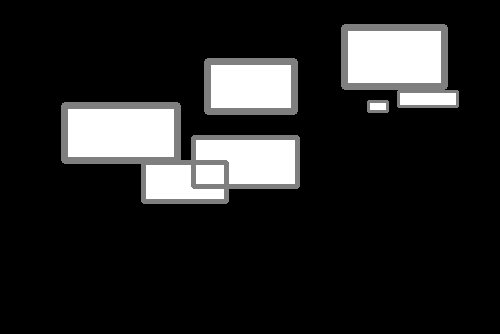
\includegraphics[width=\textwidth]{gt_branch.png}
		\caption{BranchFCN}
	\end{subfigure}
	\hfill
	\begin{subfigure}[b]{0.49\textwidth}
		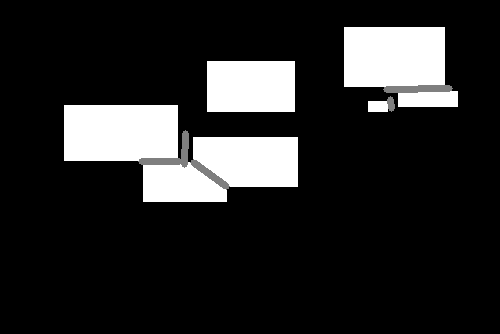
\includegraphics[width=\textwidth]{gt_word.png}
		\caption{Word Division}
	\end{subfigure}
	\caption{Immagini di groundtruth delle due varianti presentate.}
\end{figure}


\section{Finetuning e Data Augmentation}
Dopo aver cercato di migliorare l'accuratezza delle predizioni andando a modificare gli output della rete neurale e la rete stessa, per l'ottimizzazione del modello finale rimangono solo approcci quali il \textit{finetuning} e la \textit{data augmentation}, entrambi descritti nello specifico in seguito.


\subsection{Finetuning}
\label{subsec:train_fine}
Questa non è la prima volta in cui adottiamo questa tecnica, infatti come già accennato nella sezione~\ref{subsec:impl}, la parte iniziale dell'FCN da noi utilizzata fin'ora è stata sempre inizializzata con pesi derivanti da un precedente addestramento su un task generico di object classification.\par
Questo potrebbe destare dubbi sull'ottimalità dell'impostazione della rete, ma è stato ormai dimostrato come un approccio del genere sia del tutto sensato a fini di classificazione generale in più ambiti, portando a risparmiare risorse computazionali senza dover partire da un modello ex novo.\par
L'idea è dunque quella di continuare ad addestrare uno dei modelli da noi precedentemente descritti, nello specifico \textit{Word Division}, utilizzando nuovi dati provenienti da Incidental Scene Text.\par
Osservando l'andamento della curva di loss riportata nella figura~\ref{fig:finetune_loss}, i risultati appaiono ottimistici, tant'è che presto i valori vanno ad assestarsi fino a dimezzarsi dopo circa 40mila iterazioni.

\begin{figure}[H]
	\centering
	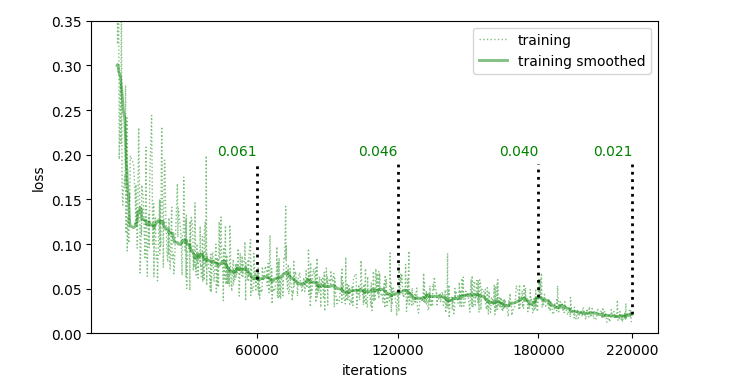
\includegraphics[width=0.95\textwidth]{finetune_loss.png}
	\caption{Curva di loss su COCO-Text prima e Incidental dopo.}
\label{fig:finetune_loss}
\end{figure}

\vfill
Purtroppo i risultati in validazione, riportati nella tabella~\ref{tab:finetune}, mostrano una realtà abbastanza diversa, anche se non a noi estranea.\par
Infatti, seppur la recall abbia un notevole incremento, lo stesso non si può dire della precision che, proprio come successo addestrando la rete da zero su Incidental Scene Text, tende a diminuire drasticamente. Ancora, questo comportamento non ha spiegazioni certe, l'unica ipotesi avanzata rimane quella della già citata differente natura delle annotazioni tra i due dataset.
\vfill

\begin{table}[H]
\centering
\begin{threeparttable}
	\begin{tabular}{l*{5}c}
		\toprule
		\multirow{2}{*}{\textbf{Iterazioni}} & \multicolumn{3}{c}{\textbf{Recall}} & \multirow{2}{*}{\textbf{Precision}} & \multirow{2}{*}{\textbf{F1-score}} \\
		\cmidrule(lr){2-4}
		& Leggibili & Illegibili & Totale &  &  \\
		\midrule
		\multicolumn{6}{l}{Intero validation set} \\
		180k		& $16.21$ & $4.14$  & $12.28$ & $13.85$ & $13.01$ \\
		220k		& $24.99$ & $11.26$ & $20.54$ & $11.95$ & $15.11$ \\
		\midrule
		\multicolumn{6}{l}{Almeno un leggibile per immagine} \\
		180k		&   ---   & $3.41$ & $12.79$ & $24.11$ & $16.71$ \\
		220k		&   ---   & $7.84$ & $21.55$ & $19.94$ & $20.72$ \\
		\bottomrule
	\end{tabular}
	\begin{tablenotes}
		\item \footnotesize{Valori espressi in percentuale.}
	\end{tablenotes}
\end{threeparttable}
\caption{}\label{tab:finetune}
\end{table}


\subsection{Data Augmentation}
\label{subsec:train_cocoaug}
Tale approccio consiste nell'aumentare la quantità di dati disponibile da fornire alla rete neurale manipolando quelli già in nostro possesso. Anche questa idea non dovrebbe giungere nuova, infatti già nell'algoritmo~\ref{alg:gendata} di generazione di ritagli randomici viene adottata una tecnica simile, in quanto per qualsiasi immagine non solo vi possono essere tanti ritagli quante le annotazioni, ma possono esservene di molteplici anche per la stessa parola.\par
Scopo di questo nuovo sviluppo è dunque quello di introdurre nuove forme di \textit{data augmentation}, illustrate nella figura~\ref{fig:data_aug}, nello specifico:
\begin{itemize}
	\item
		Scambio dei canali RGB
	\item
		Rotazione di un angolo tra $[-\theta, \theta]$
\end{itemize}

Come primo tentativo vengono applicate entrambe le trasformazioni sempre su COCO-Text, ponendo $\theta = 45\text{\textdegree}$, utilizzando una FCN base. Già i primi risultati a 60mila iterazioni riportati nella tabella~\ref{tab:cocoaug} evidenziano un comportamento già incontrato, ovvero il calo nella precisione rispetto al metodo di base.

\begin{table}[H]
\centering
\begin{threeparttable}
	\begin{tabular}{l*{5}c}
		\toprule
		\multirow{2}{*}{\textbf{Iterazioni}} & \multicolumn{3}{c}{\textbf{Recall}} & \multirow{2}{*}{\textbf{Precision}} & \multirow{2}{*}{\textbf{F1-score}} \\
		\cmidrule(lr){2-4}
		& Leggibili & Illegibili & Totale &  &  \\
		\midrule
		\multicolumn{6}{l}{Intero validation set} \\
		60k		& $15.39$ & $6.66$  & $12.53$ & $7.29$ & $9.22$ \\
		\midrule
		\multicolumn{6}{l}{Almeno un leggibile per immagine} \\
		60k		&   ---   & $5.70$ & $12.82$ & $14.53$ & $13.62$ \\
		\bottomrule
	\end{tabular}
	\begin{tablenotes}
		\item \footnotesize{Valori espressi in percentuale.}
	\end{tablenotes}
\end{threeparttable}
\caption{}\label{tab:cocoaug}
\end{table}

\begin{figure}[H]
	\centering
	\begin{subfigure}[b]{0.23\textwidth}
		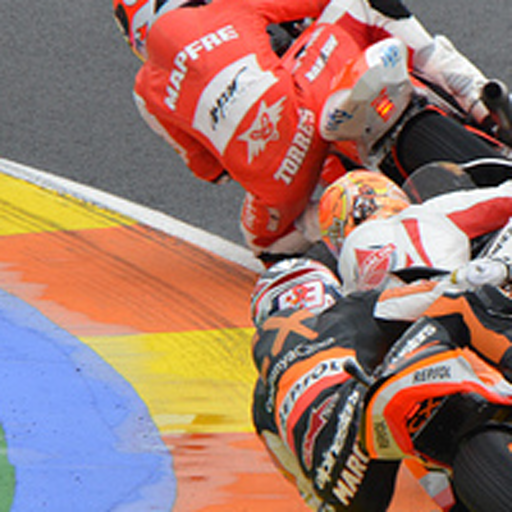
\includegraphics[width=\textwidth]{data_aug1.png}
		\caption{Originale}
	\end{subfigure}
	\hfill
	\begin{subfigure}[b]{0.23\textwidth}
		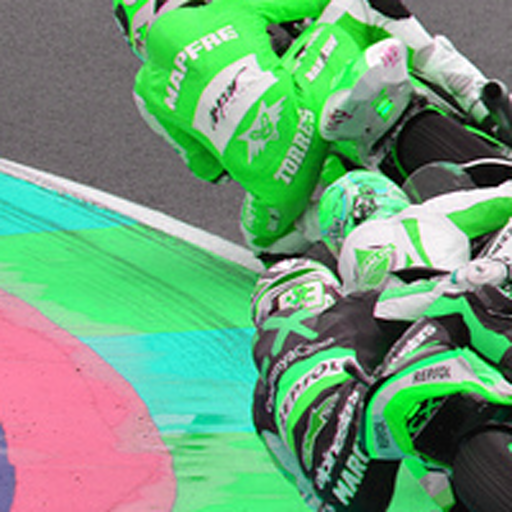
\includegraphics[width=\textwidth]{data_aug2.png}
		\caption{Scambio canali}
	\end{subfigure}
	\hfill
	\begin{subfigure}[b]{0.23\textwidth}
		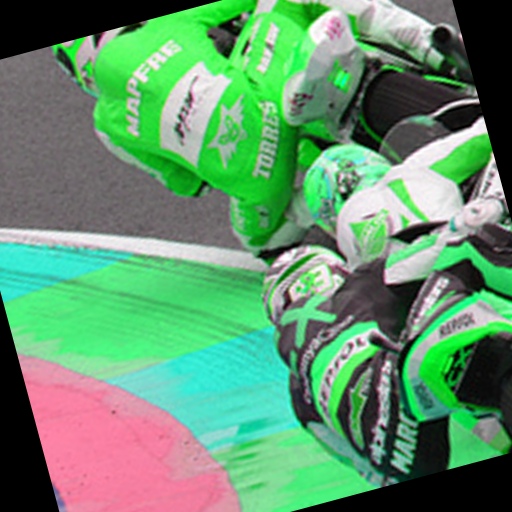
\includegraphics[width=\textwidth]{data_aug3.png}
		\caption{Rotazione}
	\end{subfigure}
\caption{}
\label{fig:data_aug}
\end{figure}


Questi risultati però ci permettono di indicare una possibile causa di questi fenomeni. Gli unici fattori imputabili sono infatti le trasformazioni applicate al dataset, e tra queste solo la rotazione potrebbe portare a somiglianze con Incidental Scene Text, il quale, a differenza di COCO-Text, presenta annotazioni precise sempre ruotate di qualche grado rispetto agli assi verticali e orizzontali.




\subsection{Confronto tra trasformazioni}
\label{subsec:train_wdaug}
Dati i risultati del precedente esperimento si è deciso di optare per questo nuovo tentativo di procedere con due approcci differenti da confrontare. 
\begin{itemize}
	\item
		Scambio canali RGB
	\item
		Scambio canali RGB + Rotazione $\theta = 15\text{\textdegree}$
\end{itemize}

La motivazione di questa scelta risiede nella volontà di testare quanto possa influire la rotazione, anche se minima, sulle performance finali. In aggiunta a ciò si passerà ad utilizzare come modello base \textit{Word Division} e l'addestramento partirà in finetuning su quest'ultimo da 120mila iterazioni fino a 180mila.\par
Confrontando i nuovi risultati nella tabella~\ref{tab:wdaug} con quelli ottenuti su \textit{Word Division} di base nella tabella~\ref{tab:word}, possiamo notare come le differenze prestazionali siano minime e come la precision tenda sempre a calare (anche se impercettibilmente con $\theta = 15\text{\textdegree}$) in favore di una migliore recall.

\begin{table}[H]
\centering
\begin{threeparttable}
	\begin{tabular}{l*{5}c}
		\toprule
		\multirow{2}{*}{\textbf{Iterazioni}} & \multicolumn{3}{c}{\textbf{Recall}} & \multirow{2}{*}{\textbf{Precision}} & \multirow{2}{*}{\textbf{F1-score}} \\
		\cmidrule(lr){2-4}
		& Leggibili & Illegibili & Totale &  &  \\
		\midrule
		\multicolumn{6}{l}{Intero validation set} \\
		Shuffle		& $38.34$ & $8.96$ & $28.52$ & $25.40$ & $26.87$ \\
		Shuffle+15	& $40.39$ & $7.78$ & $29.43$ & $24.70$ & $26.86$ \\
		\midrule
		\multicolumn{6}{l}{Almeno un leggibile per immagine} \\
		Shuffle		&   ---   & $8.40$ & $30.30$ & $37.06$ & $33.34$ \\
		Shuffle+15	&   ---   & $7.16$ & $31.34$ & $36.60$ & $33.80$ \\
		\bottomrule
	\end{tabular}
	\begin{tablenotes}
		\item \footnotesize{Valori espressi in percentuale.}
	\end{tablenotes}
\end{threeparttable}
\caption{}\label{tab:wdaug}
\end{table}


\subsection{Addestramento finale}
\label{subsec:train_final}
Infine, per l'ultimo addestramento si è deciso di utilizzare nuovamente \textit{Word Division} applicando sul dataset lo scambio dei canali RGB e la rotazione di $15\text{\textdegree}$, in quanto questo è l'approccio che fin'ora ha raggiunto risultati mediamente migliori. A differenza di quanto fatto in precedenza però il training ripartirà da zero sempre fino a 180mila iterazionni.\par
Nella tabella~\ref{tab:wdfinal} riportante i risultati finali è possibile notare come nella localizzazione di zone di aree di testo leggibili questo nuovo metodo si posizioni al di sopra di tutti gli altri, mentre complessivamente raggiunge la terza posizione, superato dai due metodi descritti nella sezione precedente~\ref{subsec:train_wdaug}. Le differenze nelle performance risultano comunque non significative. 


\begin{table}[H]
\centering
\begin{threeparttable}
	\begin{tabular}{l*{5}c}
		\toprule
		\multirow{2}{*}{\textbf{Iterazioni}} & \multicolumn{3}{c}{\textbf{Recall}} & \multirow{2}{*}{\textbf{Precision}} & \multirow{2}{*}{\textbf{F1-score}} \\
		\cmidrule(lr){2-4}
		& Leggibili & Illegibili & Totale &  &  \\
		\midrule
		\multicolumn{6}{l}{Intero validation set} \\
		180k		& $39.58$ & $9.57$ & $29.51$ & $23.66$ & $26.26$ \\
		\midrule
		\multicolumn{6}{l}{Almeno un leggibile per immagine} \\
		180k		&   ---   & $8.99$ & $31.34$ & $36.84$ & $33.87$ \\
		\bottomrule
	\end{tabular}
	\begin{tablenotes}
		\item \footnotesize{Valori espressi in percentuale.}
	\end{tablenotes}
\end{threeparttable}
\caption{}\label{tab:wdfinal}
\end{table}


In conclusione è possibile affermare come gli ultimi tentativi di \textit{data augmentation} abbiano portato miglioramenti negligibili in quanto le operazioni applicate sono poco significative rispetto a quanto già fatto nel modello base con l'utilizzo dei ritagli dettati dalle annotazioni. 


\subsection{Tabelle riassuntive}
Di seguito riportati i risultati dei vari metodi sviluppati mostrando:
\begin{itemize}
	\item
		recall, precision e F1-score totali (tabella~\ref{tab:total_results})
	\item
		recall, precision, e F1-score solo su annotazioni leggibili (tabella~\ref{tab:legible_results})
	\item
		recall specifica per le varie classi (tabella~\ref{tab:results_recall})
\end{itemize}

\vfill

\begin{table}[H]
\centering
\resizebox{\columnwidth}{!}{%
\begin{threeparttable}
	\begin{tabular}{l *{2}c *{2}c >{\bf}c }
		\toprule
		
		\textbf{Dataset} & \textbf{Metodo} & \textbf{Iters}	&
		\textbf{Recall} & \textbf{Precision} & \textbf{F1-score} \\

		\midrule

		Incidental Scene Text & FCN & 60k
			& 14.54 & 7.87 & 10.21 \\ 
		COCO Shuffled 45\textdegree{} & FCN & 60k
			& 12.53 & 7.29 & 9.22 \\ 
		COCO-Text & FCN & 60k
			& 12.28 & 13.85 & 13.01 \\ 
		COCO-Text & FCN & 180k
			& 17.29 & 17.72 & 17.50 \\ 
		COCO + Incidental & FCN & 220k
			& 20.54 & 11.95 & 15.11 \\ 
		COCO-Text & BranchFCN & 180k
			& 26.13 & 21.55 & 23.62 \\ 
		COCO-Text & WordDivision & 180k
			& 28.70 & 23.64 & 25.94 \\ 
		COCO Shuffled & WordDivision & 180k
			& 28.52 & 25.40 & 26.87 \\ 
		COCO Shuffled 15\textdegree{} & WordDivision & 180k
			& 29.43 & 24.70 & 26.86 \\ 
		COCO Shuffled 15\textdegree{} & WordDivision & 180k	
			& 29.51 & 23.66 & 26.26 \\

		\bottomrule
	\end{tabular}
	\begin{tablenotes}
		\item \footnotesize{Valori espressi in percentuale.}
	\end{tablenotes}
\end{threeparttable}%
}
\caption{Risultati sull'intero validation set.}\label{tab:total_results}
\end{table}

\vfill

\begin{table}[H]
\centering
\resizebox{\columnwidth}{!}{%
\begin{threeparttable}
	\begin{tabular}{l *{2}c *{2}c >{\bf}c }
		\toprule
		
		\textbf{Dataset} & \textbf{Metodo} & \textbf{Iters}	&
		\textbf{Recall} & \textbf{Precision} & \textbf{F1-score} \\

		\midrule

		Incidental Scene Text & FCN & 60k
			& 15.48 & 13.95 & 14.67 \\ 
		COCO Shuffled 45\textdegree{} & FCN & 60k
			& 12.82 & 14.53 & 13.62 \\ 
		COCO-Text & FCN & 60k
			& 12.79 & 24.11 & 16.71 \\ 
		COCO-Text & FCN & 180k
			& 17.78 & 28.15 & 21.79 \\ 
		COCO + Incidental & FCN & 220k
			& 21.55 & 19.94 & 20.72 \\ 
		COCO-Text & BranchFCN & 180k
			& 27.99 & 35.46 & 31.29 \\ 
		COCO-Text & WordDivision & 180k
			& 30.60 & 36.74 & 33.39 \\ 
		COCO Shuffled & WordDivision & 180k
			& 30.30 & 37.06 & 33.34 \\ 
		COCO Shuffled 15\textdegree{} & WordDivision & 180k
			& 31.40 & 36.60 & 33.80 \\ 
		COCO Shuffled 15\textdegree{} & WordDivision & 180k	
			& 31.34 & 36.84 & 33.87 \\

		\bottomrule
	\end{tabular}
	\begin{tablenotes}
		\item \footnotesize{Valori espressi in percentuale.}
	\end{tablenotes}
\end{threeparttable}%
}
\caption{Risultati sulle sole annotazioni leggibili.}\label{tab:legible_results}
\end{table}

\vfill

\begin{sidewaystable}
\begin{table}[H]
\centering
\resizebox{\columnwidth}{!}{%
\begin{threeparttable}
	\begin{tabular}{l *{5}c >{\it\/}c *{3}c >{\it\/}c >{\bf}c }
		\toprule
		
		\multirow{3}{*}{\textbf{Dataset}}		&
		\multirow{3}{*}{\textbf{Metodo}}		&
		\multirow{3}{*}{\textbf{Iters}}			&
		\multicolumn{9}{c}{\textbf{Recall}}		\\

		\cmidrule(lr){4-12}
		& & & \multicolumn{4}{c}{Leggibili} & \multicolumn{4}{c}{Illeggibili} & \multirow{2}{*}{} \\ 

		\cmidrule(lr){4-7} \cmidrule(lr){8-11} 

		& & & MP$^1$ & HW$^2$ & OT$^3$ & & MP$^1$ & HW$^2$ & OT$^3$ & & \\ 

		\midrule

		Incidental Scene Text & FCN & 60k
			& 19.40 & 15.51 & 12.78 & 19.07 & 6.13 & 7.10 & 4.14 & 5.78 & 14.54 \\
		COCO Shuffled 45\textdegree{} & FCN & 60k
			& 15.46 & 14.78 & 13.57 & 15.39 & 7.27 & 9.51 & 3.73 & 6.66 & 12.53 \\
		COCO-Text & FCN & 60k
			& 16.56 & 10.78 & 12.72 & 16.21 & 4.57 & 6.04 & 2.03 & 4.14 & 12.28 \\
		COCO-Text & FCN & 180k
			& 21.13 & 16.15 & 19.39 & 20.87 & 10.72 & 10.17 & 5.05 & 9.59 & 17.29 \\
		COCO + Incidental & FCN & 220k
			& 25.31 & 20.54 & 20.73 & 24.99 & 12.29 & 13.06 & 6.95 & 11.26 & 20.54 \\
		COCO-Text & BranchFCN & 180k
			& 36.36 & 30.66 & 27.61 & 35.91 & 7.94 & 7.48 & 3.19 & 6.98 & 26.13 \\
		COCO-Text & WordDivision & 180k
			& 39.61 & 31.10 & 24.17 & 38.88 & 9.37 & 10.34 & 4.15 & 8.37 & 28.70 \\
		COCO Shuffled & WordDivision & 180k
			& 39.00 & 30.88 & 25.42 & 38.34 & 9.72 & 13.10 & 5.01 & 8.96 & 28.52 \\
		COCO Shuffled 15\textdegree{} & WordDivision & 180k
			& 41.01 & 33.33 & 28.73 & 40.39 & 8.59 & 9.38 & 4.29 & 7.78 & 29.43 \\
		COCO Shuffled 15\textdegree{} & WordDivision & 180k	
			& 40.18 & 32.84 & 28.33 & 39.58 & 10.55 & 12.00 & 5.25 & 9.57 & 29.51 \\

		\bottomrule
	\end{tabular}
	\begin{tablenotes}
		\item \footnotesize{Valori espressi in percentuale.}
		\item \footnotesize{$^1$ Machine Printed}
		\item \footnotesize{$^2$ Handwritten}
		\item \footnotesize{$^3$ Others}
	\end{tablenotes}
\end{threeparttable}%
}
\caption{Valori di recall per le diverse classi.}\label{tab:results_recall}
\end{table}
\end{sidewaystable}


\section{Confronto con lo stato dell'arte}
In quest'ultima parte verranno mostrati i risultati ottenuti sui test set a disposizione al fine di mettere alla prova i modelli da noi addestrati contro metodi sviluppati da terzi negli ultimi anni.\par
Dalla nostra parte, i modelli presi in considerazione sono: 
\begin{itemize}
	\item
		BranchFCN (sezione~\ref{subsec:train_branch})
	\item
		Word Division con dataset aumentato (sezione~\ref{subsec:train_final})
	\item
		BranchFCN con soglia 0.65 e doppia \texttt{dilation}
	\item
		Word Division con dataset aumentato con soglia 0.6
\end{itemize}

Gli ultimi due modelli citati non sono stati prima analizzati in quanto sono variazioni nate nel corso di questi ultimi test al fine di massimizzare le prestazioni su Incidental Scene Text. In aggiunta a ciò, gli input della rete sono ridimensionati a risoluzioni vicine a \texttt{640 $\times$ 480}, media delle immagini di COCO-Text, in quanto alte risoluzioni portano ad una perdita di accuratezza facendo risaltare dettagli fuorvianti.\par
Come già accennato i test set sono quelli di \textit{Incidental Scene Text} e \textit{Focused Scene Text}, mentre i metodi di terzi riportati saranno quelli dei vincitori delle rispettive edizioni di ICDAR (2015 e 2013 rispettivamente) più i vari contendenti che hanno ottenuti i migliori risultati durante le successive edizioni, seppur non ufficialmente.

\subsection{Incidental Scene Text}

\begin{table}[H]
\centering
\begin{threeparttable}
	\begin{tabular}{l *{2}c >{\bf}c }
		\toprule
		
		\textbf{Metodo} & \textbf{Recall} & \textbf{Precision} & \textbf{F1-score} \\

		\midrule

		BranchFCN
		& 33.75 & 44.34 & 38.33 \\
		BranchFCN Tweaked
		& 37.02 & 54.19 & 43.99 \\
		WordDivision
		& 34.52 & 38.65 & 36.47 \\
		WordDivision Tweaked
		& 35.29 & 42.62 & 38.61 \\
		\midrule

		\multicolumn{1}{r}{Top-4 2015~\cite{ICDAR2015results}} \\
		Stradvision-2
		& 36.74 & 77.46 & 49.84 \\
		StradVision-1
		& 46.27 & 53.39 & 49.57 \\
		NJU Text (Version2)	
		& 36.25 & 70.44 & 47.87 \\
		AJOU~\cite{ajou}
		& 46.94 & 47.26 & 47.10 \\
		\midrule

		\multicolumn{1}{r}{Top-3 2017~\cite{ICDAR2015results}} \\
		Baidu VIS
		& 83.39 & 93.62 & 88.21 \\
		SenseTime V3 
		& 84.83 & 90.82 & 87.73 \\
		Dahua-OCR V3
		& 83.44 & 91.31 & 87.19 \\

		\bottomrule
	\end{tabular}
	\begin{tablenotes}
		\item \footnotesize{Valori espressi in percentuale.}
	\end{tablenotes}
\end{threeparttable}
\caption{Risultati sull'intero validation set.}\label{tab:incidental_results}
\end{table}

Dai risultati riporati nella tabella~\ref{tab:incidental_results} è possibile notare come nel giro di pochi anni lo stato dell'arte sia avanzato in maniera considerevele, ma è doveroso sottolineare come i nostri risultati ottenuti con strumenti disponibili al pubblico già nel 2015, ci possano posizionare nella classifica di quell'anno in quinta posizione con \textit{BranchFCN Tweaked}, oppure in settima con il modello con parametri di base.\par
Da notare è l'inversione di performance tra \textit{BranchFCN} e \textit{Word Division} rispetto ai risultati ottenuti su COCO-Text in fase di validazione, soprattutto nelle loro versioni migliorate.

\subsection{Focused Scene Text}

\begin{table}[H]
\centering
\begin{threeparttable}
	\begin{tabular}{l *{2}c >{\bf}c }
		\toprule
		
		\textbf{Metodo} & \textbf{Recall} & \textbf{Precision} & \textbf{F1-score} \\

		\midrule

		BranchFCN
		& 66.03 & 59.95 & 62.84 \\	
		BranchFCN Tweaked
		& 74.52 & 66.61 & 70.34 \\
		WordDivision
		& 67.21 & 57.54 & 62.01 \\
		WordDivision Tweaked
		& 70.96 & 59.40 & 64.67 \\
		\midrule

		\multicolumn{1}{r}{Top-3 2013~\cite{ICDAR2013results}} \\
		2R\_NUS\_FAR
		& 68.95 & 74.46 & 71.60 \\
		USTB\_TexStar
		& 61.46 & 84.76 & 71.25 \\
		CASIA\_NLPR
		& 66.12 & 74.64 & 70.12 \\
		\midrule

		\multicolumn{1}{r}{Top-3 2015~\cite{ICDAR2013results}} \\
		VGGMaxNet\_cmb~\cite{vggmaxnet}
		& 78.08 & 90.09 & 83.66 \\
		VGGMaxNet\_025~\cite{vggmaxnet}
		& 79.82 & 87.58 & 83.52 \\
		VGGMaxNet\_013~\cite{vggmaxnet}
		& 76.53 & 90.50 & 82.93 \\
		\midrule

		\multicolumn{1}{r}{Top-3 2017~\cite{ICDAR2013results}} \\	
		SenseTime
		& 91.87 & 95.45 & 93.62 \\
		DLVCtext
		& 88.49 & 93.35 & 90.86 \\
		MultDet
		& 89.68 & 91.09 & 90.38 \\

		\bottomrule
	\end{tabular}
	\begin{tablenotes}
		\item \footnotesize{Valori espressi in percentuale.}
	\end{tablenotes}
\end{threeparttable}
\caption{Risultati sull'intero validation set.}\label{tab:focused_results}
\end{table}

Similmente a quanto osservato su Incidental Scene Text, nel tempo lo stato dell'arte è notevolmente avanzato e \textit{BranchFCN} è ancora in netto vantaggio rispetto a \textit{Word Division}, anche se solo nella sua versione modificata.\par
Questa volta però i nostri approcci non raggiungono risultati soddisfacenti, posizionandosi poco dietro i primi classificati nel 2013, ma ben lontani dai modelli concorrenti sviluppati fino al 2015.

